\documentclass[a4paper,12pt,final]{article}


\usepackage{graphicx}
\title{
\begin{center}
  	
\includegraphics[scale=0.3]{Logo.png} 
  \end{center}
  \textbf{\\}
Iteration 2\\
}
\author{101 Solutions}

\begin{document}

\maketitle
\thispagestyle{empty}
\newpage
\tableofcontents
\thispagestyle{empty}
\newpage
\pagenumbering{arabic}

\section{Introduction}
The purpose of this document is to keep track of the ongoing development progress of the software application manager AppMan.  In each iteration additional content will be added which will result in this document being an up to date and relaible method to view progress and current development plans and ideas. Content will include milestones reached, current goals and the current functionality of the software.

\section{Milestones reached}
\begin{itemize}
\item A cleaner GUI implementation
\item A reliable socket connection(Tcp) between the server and client applications, which will serve as a communication pathway
\item Build Copy from master to slave(Logically)
\item View builds on the master including further information that can be displayed
\item An expandible communication protocol which will be expanded to include new and further functionality
\item Creating a database that can store information related to builds kept on the master and slaves
\item MD5 sum generation to determine if there is a difference between the build on Master Machine and Slave Machine
\item Colour coding to display if builds on master or slave machine have similar content(Green, Yellow, Red)
\end{itemize}


\section{Immediate Goals}
Our next main goals for the project:
\subsection{Build transference}
\begin{itemize}
\item Goal: The ability to copy the builds to the clients(Slave computers) and also to compress the files that will be copied
\end{itemize}
\subsection{Build Information Comparison}
\begin{itemize}
\item Goal: The ability to synchronize two builds on master and slave computers(i.e. if a change have been made to a file)
\end{itemize}
\subsection{Slave System Information}
\begin{itemize}
\item Goal: The ability to transfer system information to master and back
\end{itemize}


\section{System Design}
\subsection{AppMan}

\begin{center}
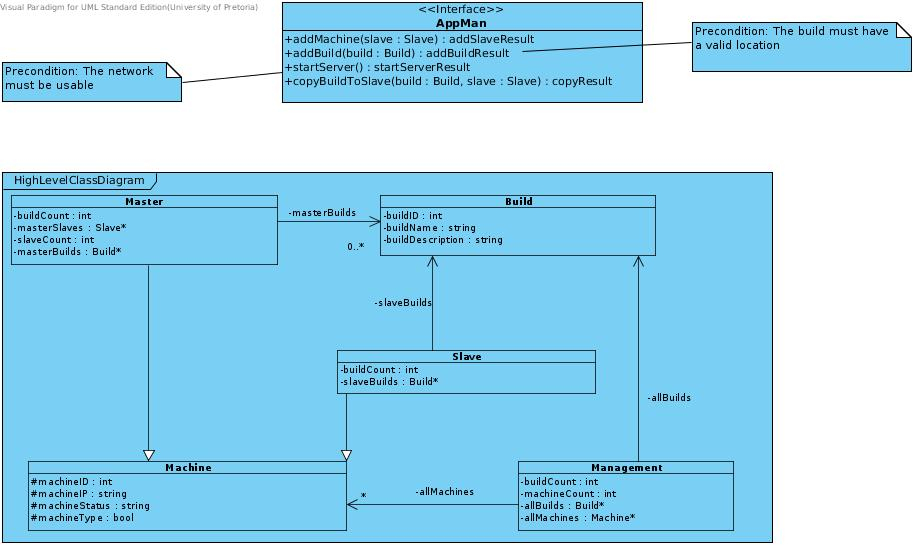
\includegraphics[scale=0.5]{AppManDiagram.jpg} 
\end{center}

\newpage
\begin{center}
Detailed Class Diagram(AppMan)
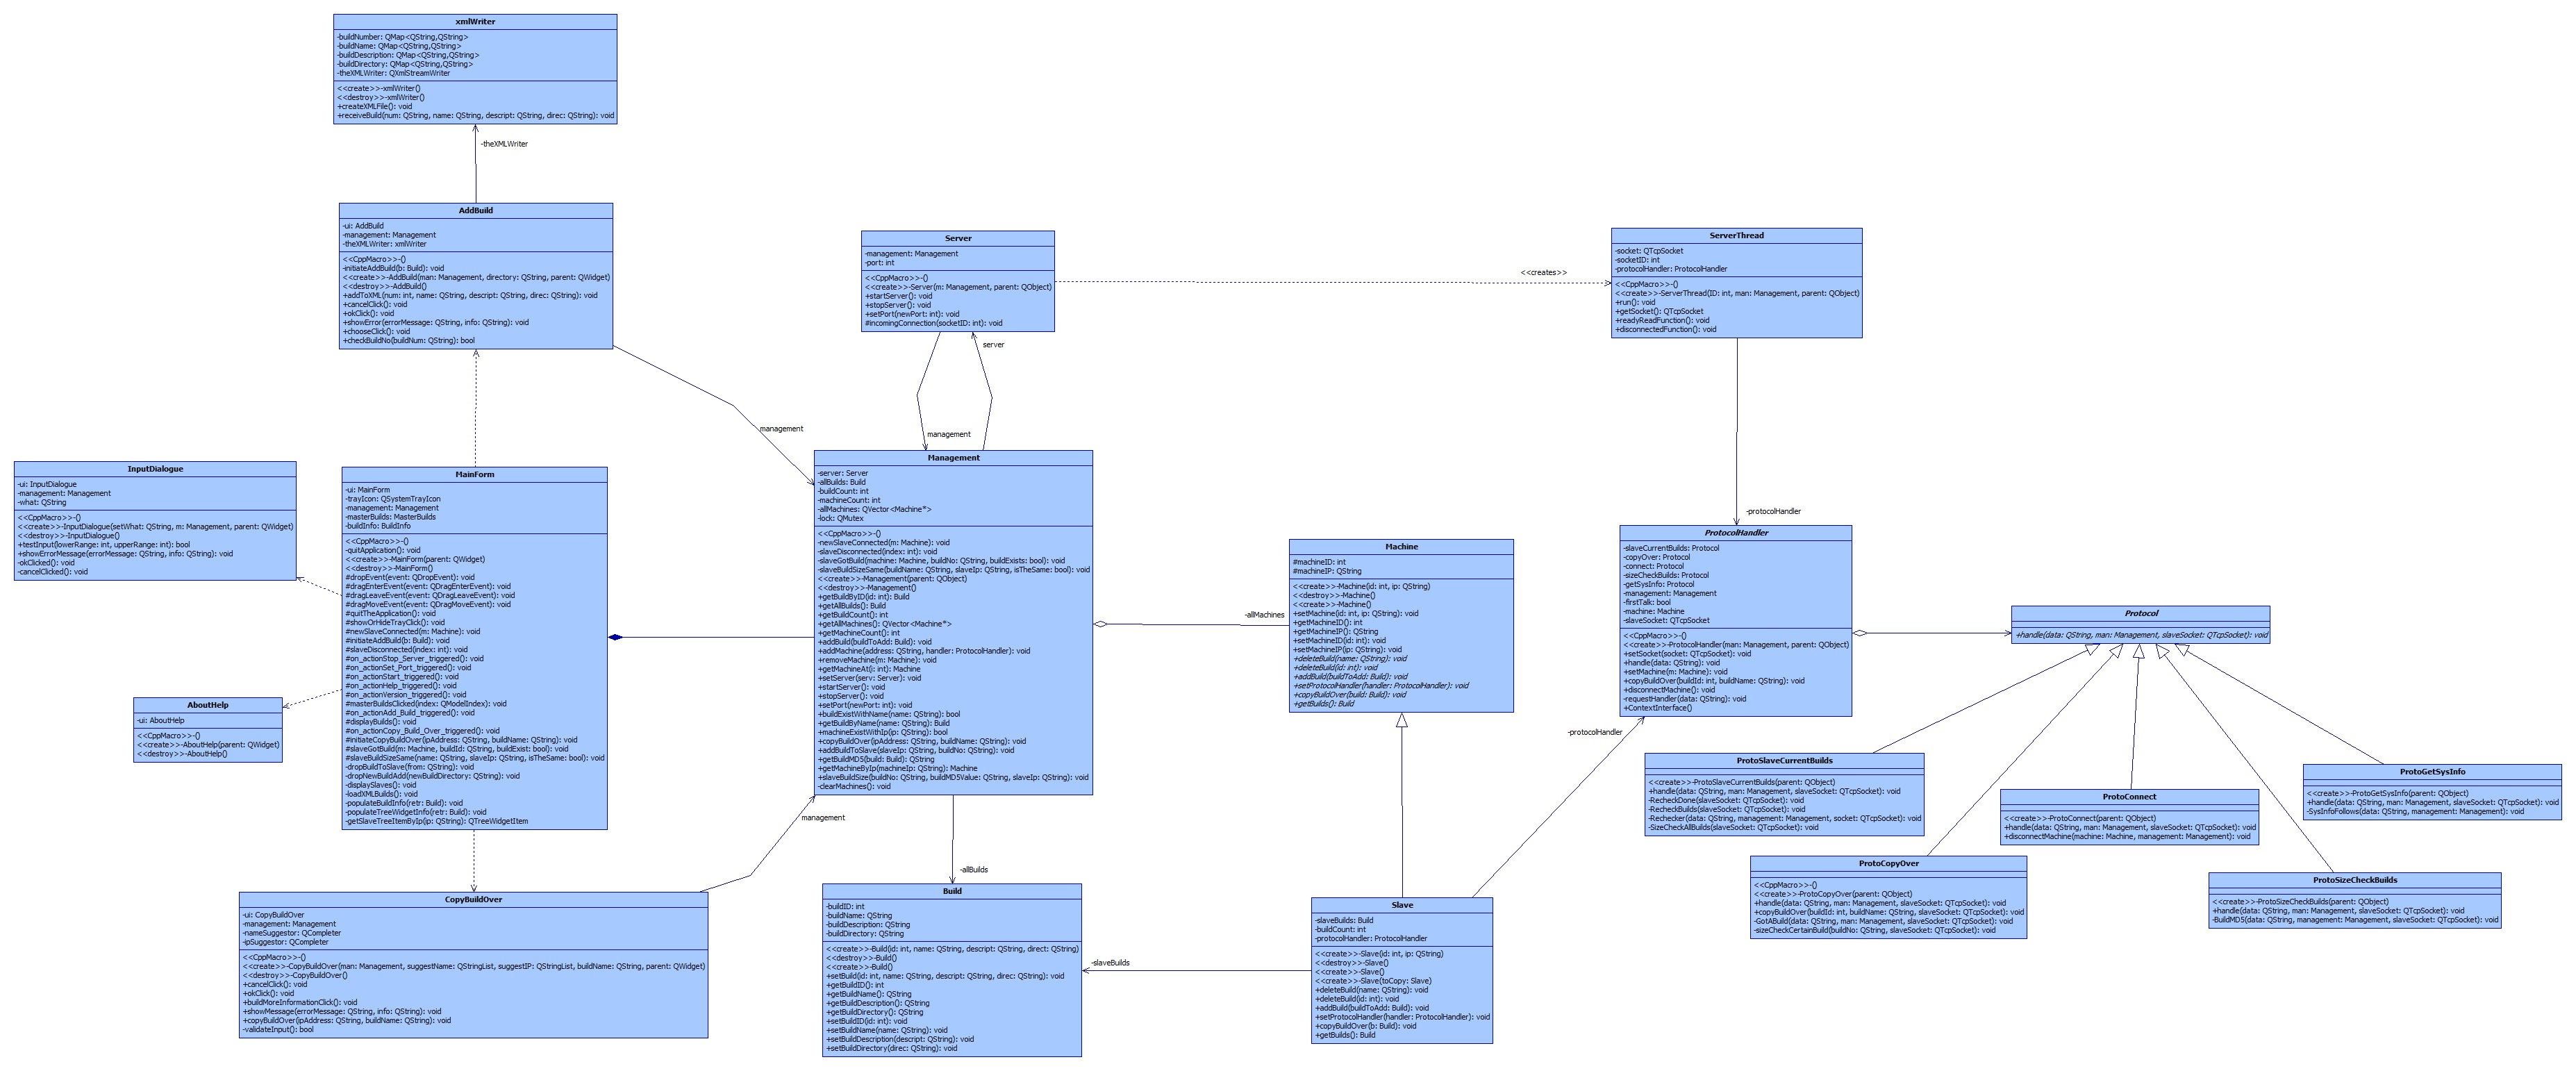
\includegraphics[angle = 90, height=20cm]{ClassDiagramAppMan.jpg} 
\end{center}

\subsection{AppManClient}

\begin{center}
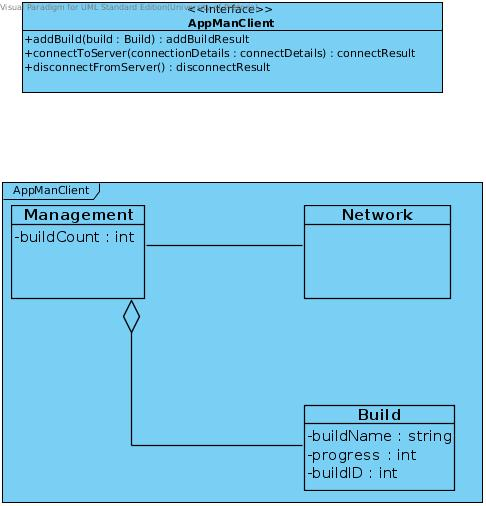
\includegraphics[scale=0.5]{AppManClientDiagram.jpg} 
\end{center}

\newpage
\begin{center}
Detailed Class Diagram(AppManClient)
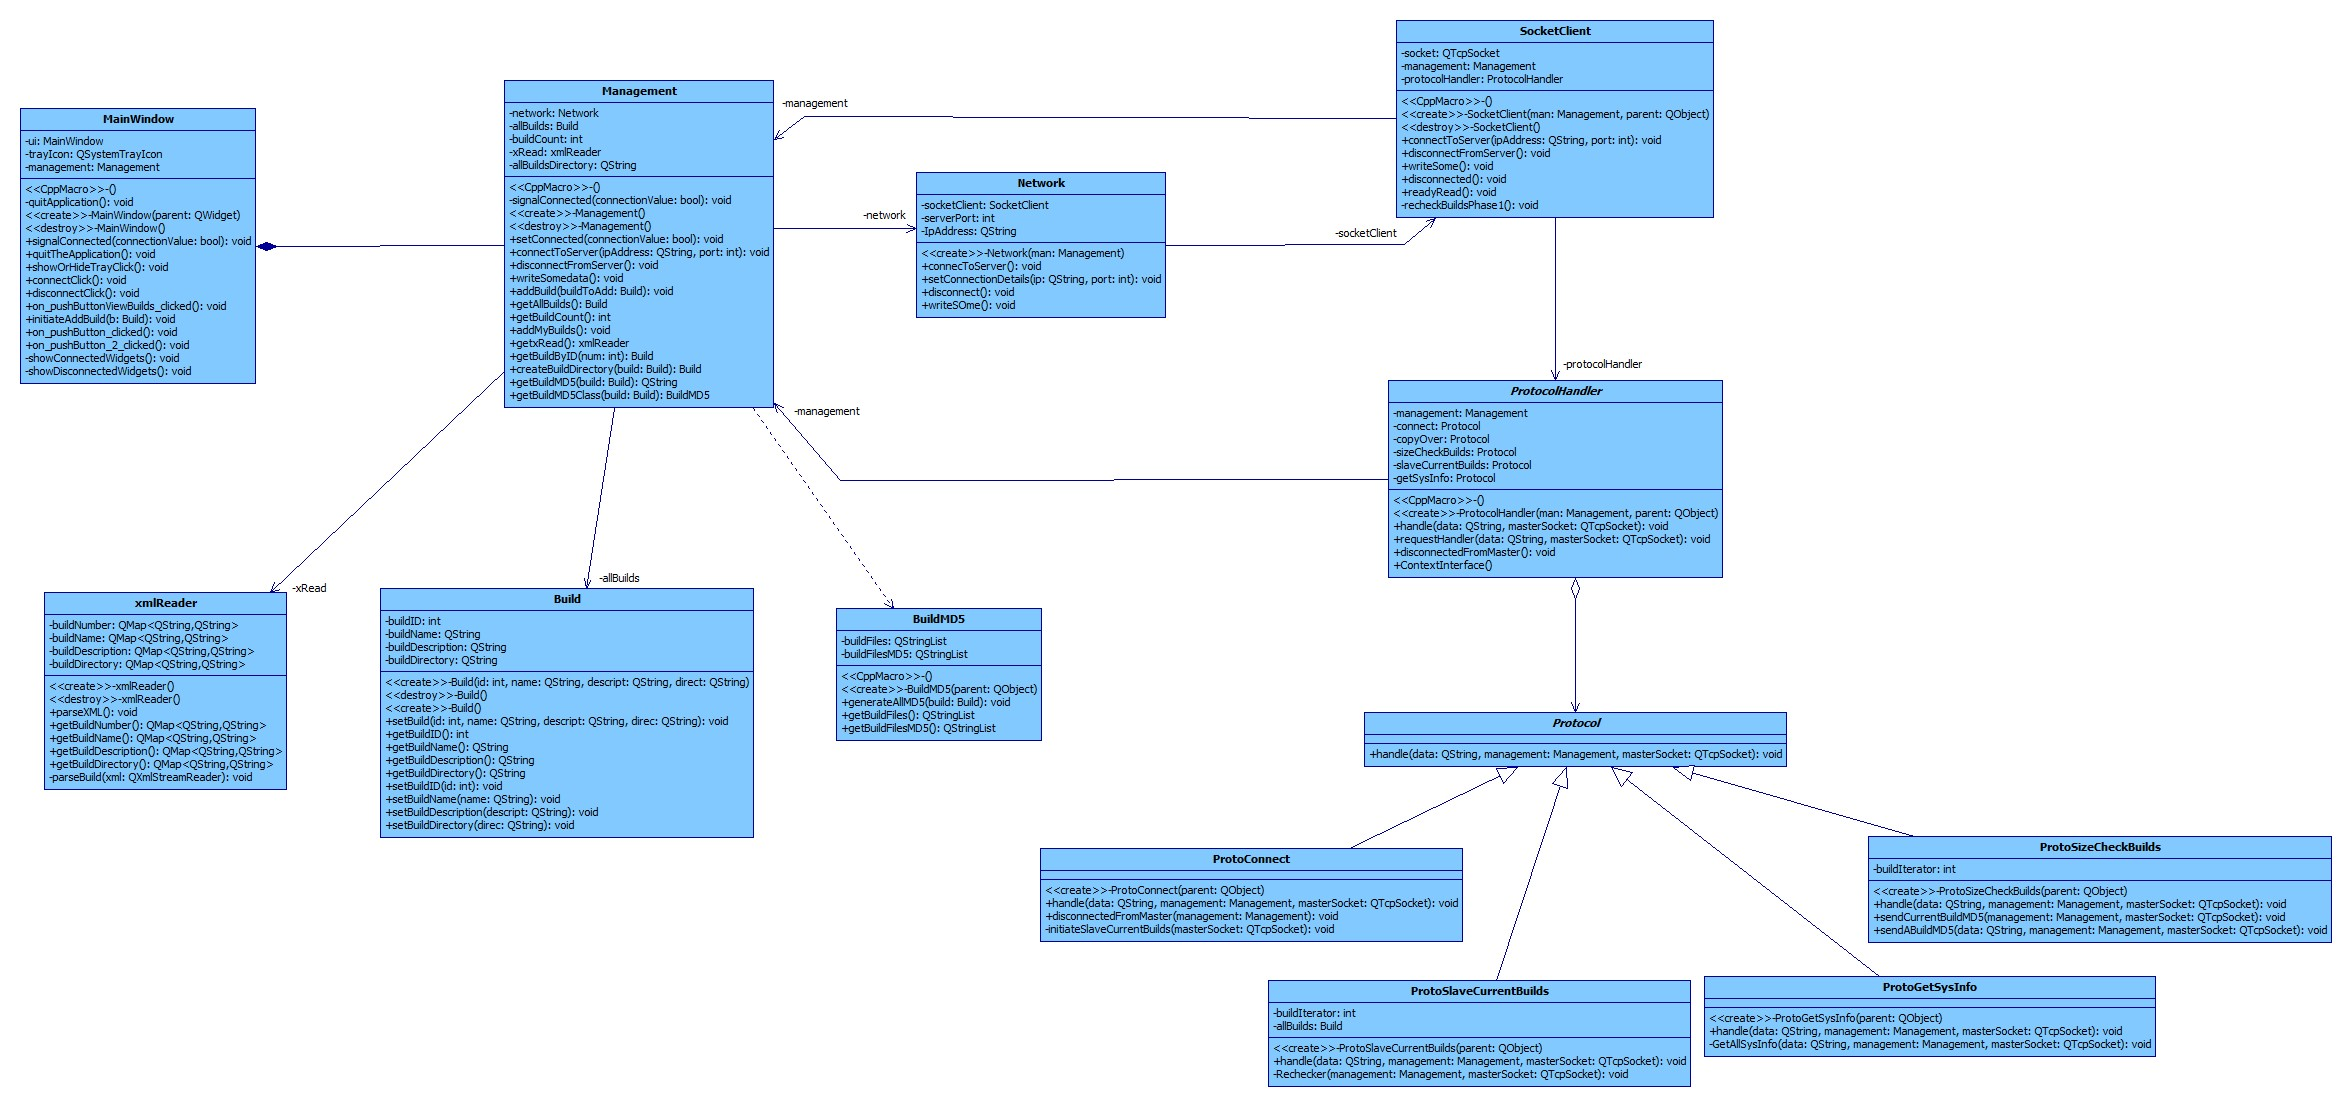
\includegraphics[angle = 90, height=20cm]{ClassDiagramAppManClient.jpg} 
\end{center}

\section{Processes}
\subsection{ActivityDiagram}
\begin{center}
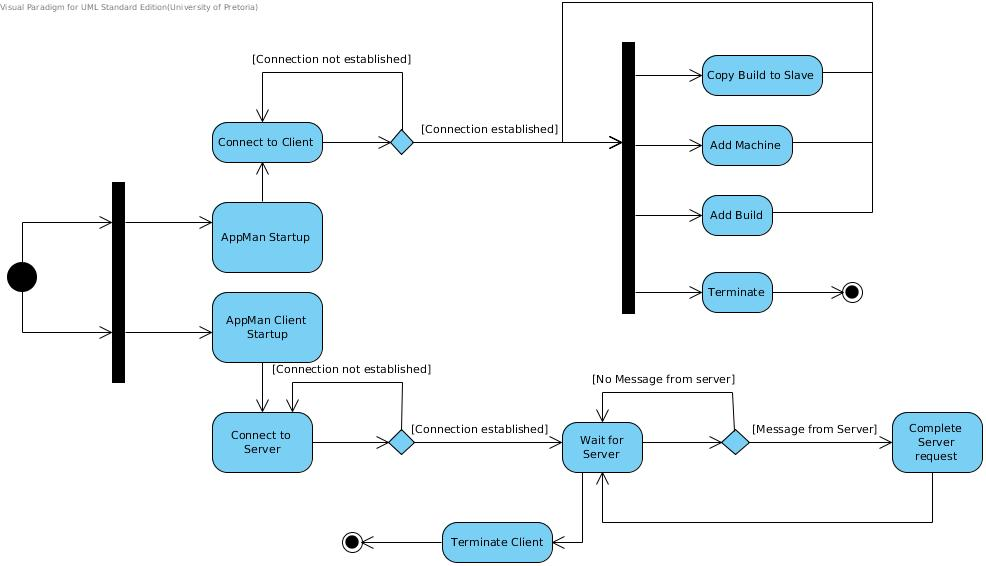
\includegraphics[scale=0.38]{ActivityDiagram.jpg} 
\end{center}
\subsection{Add Build ActivityDiagram}
\begin{center}
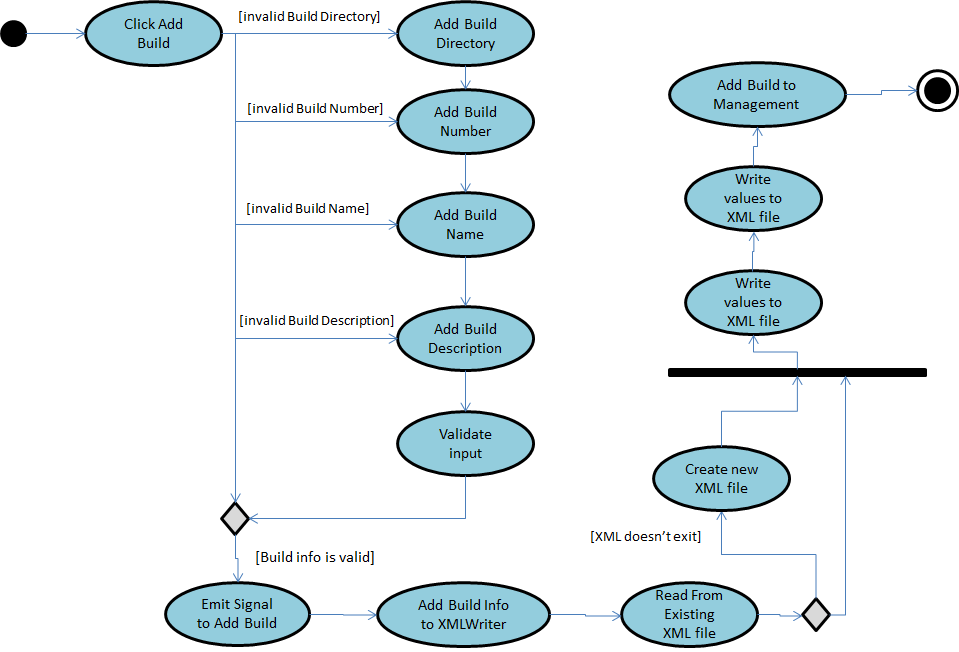
\includegraphics[scale=0.45]{AddBuildActivity.png} 
\end{center}
\subsection{Get System Info ActivityDiagram}
\begin{center}
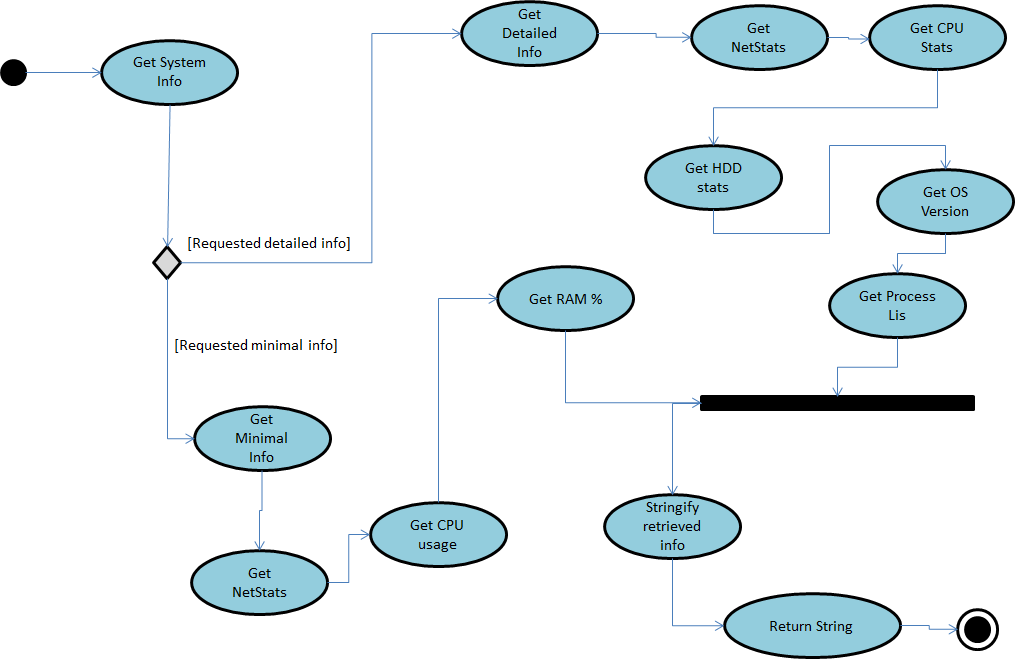
\includegraphics[scale=0.45]{GetSystemInfo.png} 
\end{center}

\section{Communication Protocol}
Brief Description: The following diagrams are Data Flow Diagrams describing the protocol that is used to implement communication between the AppMan and AppManClient. The protocol is easy to understand and each of them serve a purpose in order to harbour proper communication. The order in which the communication takes place are indicated by the numbers near the flow.
\vspace{12pt}\newline
%Note: while not all the functions are shown in the sequence diagrams, they merely serve as a simple representation to find out how the communication takes place. Furthermore after the Connect protocol are followed, most of the classes are initialized along with all the required variables.

%%%%%%%%%%%%%%%%%%%%%%%
%%%%%%CONNECT			(Begin)
%%%%%%%%%%%%%%%%%%%%%%%
\subsection{Connect}
This protocol is followed when the client application first connects to the AppMan server. The connecting application will directly be disconnected if the correct protocol is not followed. SlaveCurrentBuilds protocol directly follows this protocol.
\begin{center}
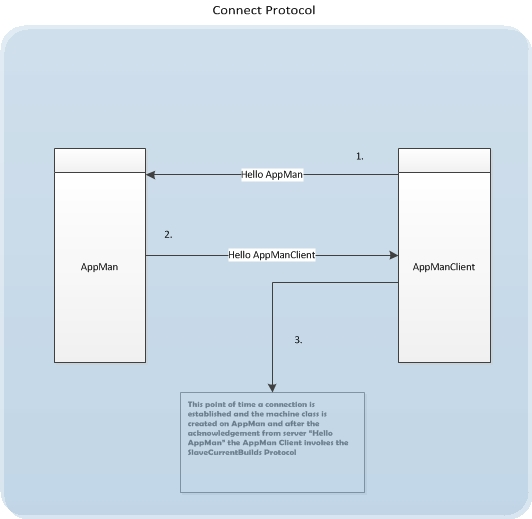
\includegraphics[scale=1.0]{CommunicationProtocol/ConnectProtocol.jpg} 
\end{center}

%\newpage
%\begin{center}
%Sequence Diagram(For Client Application)
%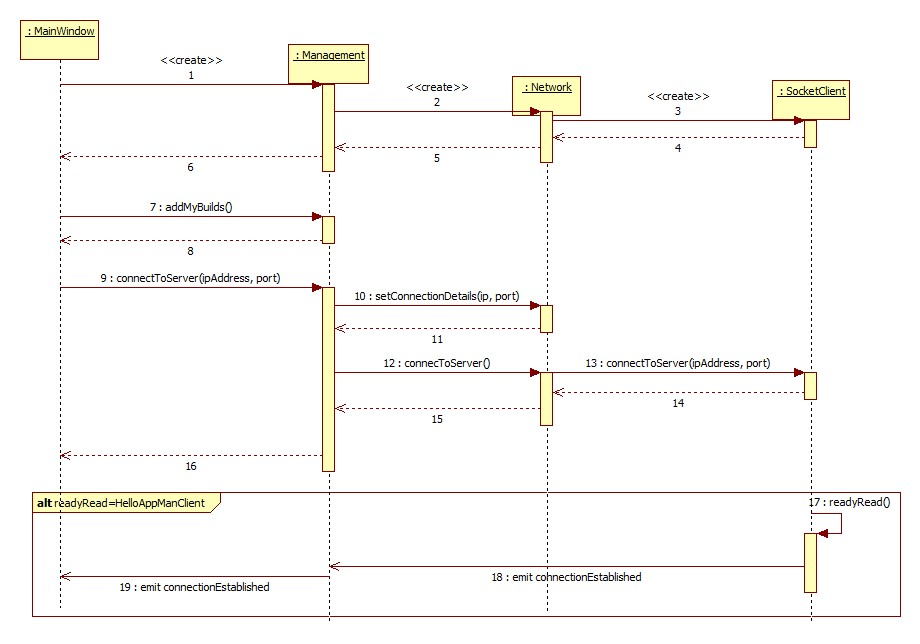
\includegraphics[scale=0.4]{CommunicationProtocol/SequenceDiagrams/Client/Connect.jpg} 
%\end{center}
%\begin{center}
%Sequence Diagram(For Master Application)
%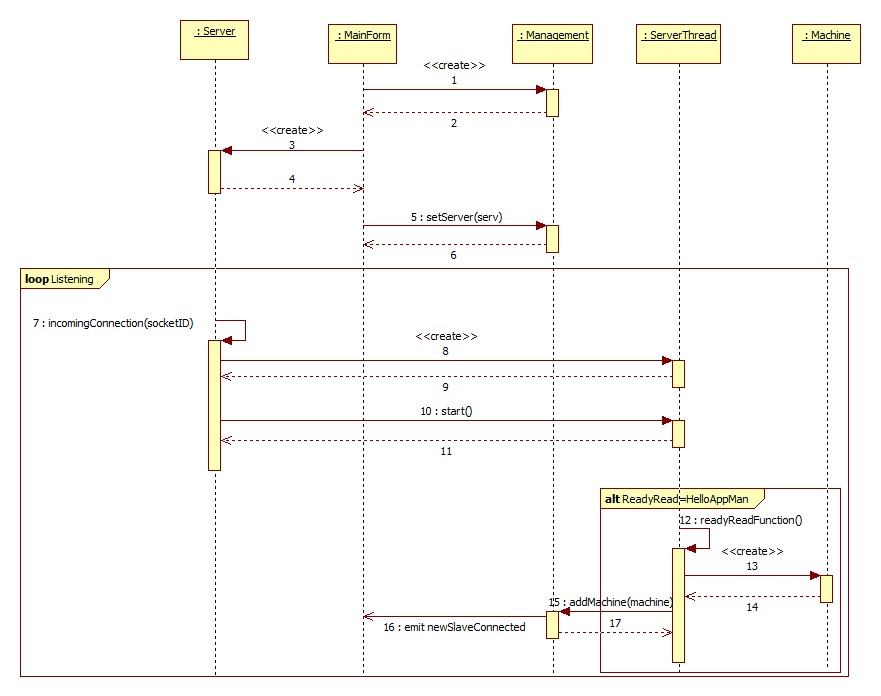
\includegraphics[scale=0.4]{CommunicationProtocol/SequenceDiagrams/Server/Connect.jpeg} 
%\end{center}
%%%%%%%%%%%%%%%%%%%%%%%
%%%%%%CONNECT			(End)
%%%%%%%%%%%%%%%%%%%%%%%


%%%%%%%%%%%%%%%%%%%%%%%
%%%%%%SlaveCurrentBuilds(Begin)
%%%%%%%%%%%%%%%%%%%%%%%
\subsection{SlaveCurrentBuilds}
This protocol is invoked directly after Connect protocol and will update all the builds that are currently on the slave and show them on the master. With this protocol one can see all the builds that are there. Apon reaching the "RecheckDone" data, the SizeCheckBuilds protocol will be invoked for each build.
\begin{center}
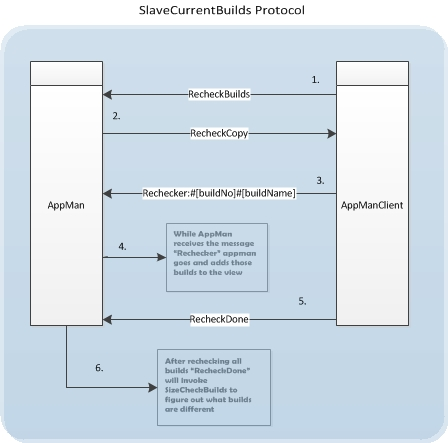
\includegraphics[scale=1.0]{CommunicationProtocol/SlaveCurrentBuildsProtocol.jpg} 
\end{center}

%\newpage
%\begin{center}
%Sequence Diagram(For Client Application)
%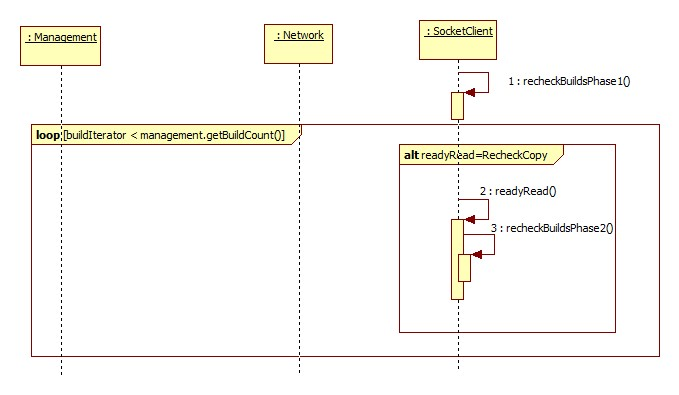
\includegraphics[scale=0.5]{CommunicationProtocol/SequenceDiagrams/Client/SlaveCurrentBuilds.jpg} 
%\end{center}
%\begin{center}
%Sequence Diagram(For Master Application)
%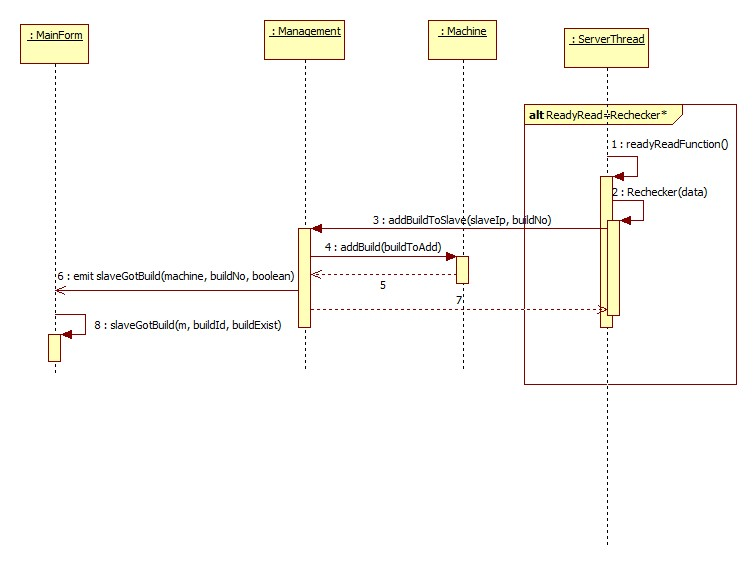
\includegraphics[scale=0.5]{CommunicationProtocol/SequenceDiagrams/Server/SlaveCurrentBuilds.jpeg} 
%\end{center}
%%%%%%%%%%%%%%%%%%%%%%%
%%%%%%SlaveCurrentBuilds(End)
%%%%%%%%%%%%%%%%%%%%%%%



%%%%%%%%%%%%%%%%%%%%%%%
%%%%%%SizeCheckBuilds		(Begin)
%%%%%%%%%%%%%%%%%%%%%%%
\subsection{SizeCheckBuilds}
This protocol is followed when determining if the build of the AppMan and AppManClient have different MD5 values which will indicate that there are differences in the builds themself. If a difference is detected CopyOver protocol is invoked to copy the build files over from the Master machine to Slave Machine.
\begin{center}
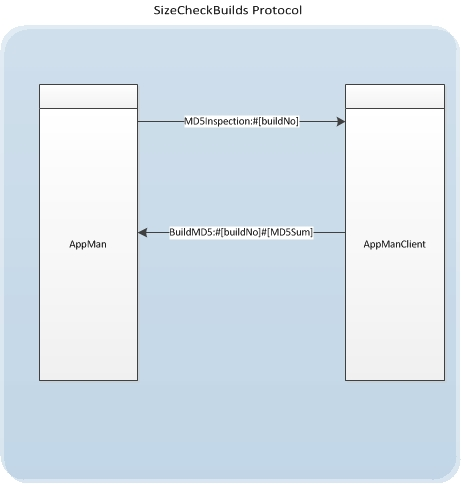
\includegraphics[scale=1.0]{CommunicationProtocol/SizeCheckBuildsProtocol.jpg} 
\end{center}

%%%%%%%%%%%%%%%%%%%%%%%
%%%%%%SizeCheckBuilds		(End)
%%%%%%%%%%%%%%%%%%%%%%%




%%%%%%%%%%%%%%%%%%%%%%%
%%%%%%CopyOver			(Begin)
%%%%%%%%%%%%%%%%%%%%%%%
\subsection{CopyOver}
This protocol is followed when a build is logically copied over from master to slave. The build name and number is saved on the slave side. 
\begin{center}
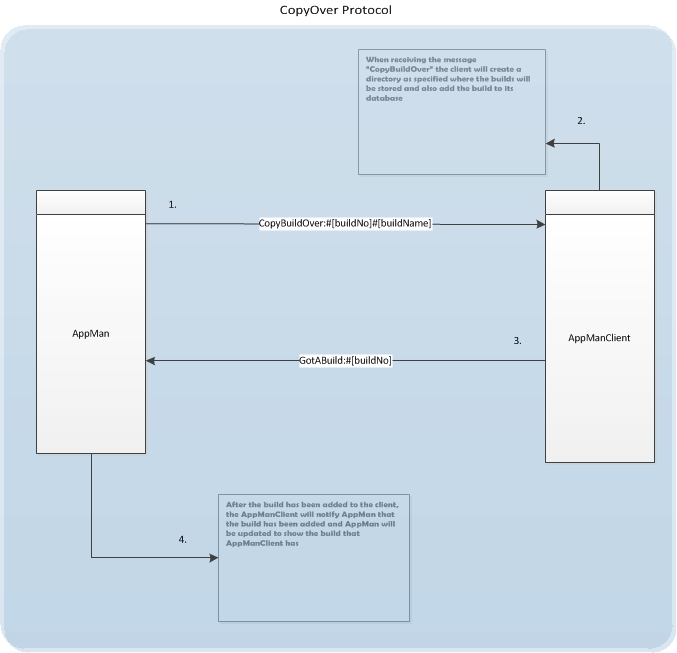
\includegraphics[scale=0.85]{CommunicationProtocol/CopyOverProtocol.jpg} 
\end{center}


%\newpage
%\begin{center}
%Sequence Diagram(For Client Application)
%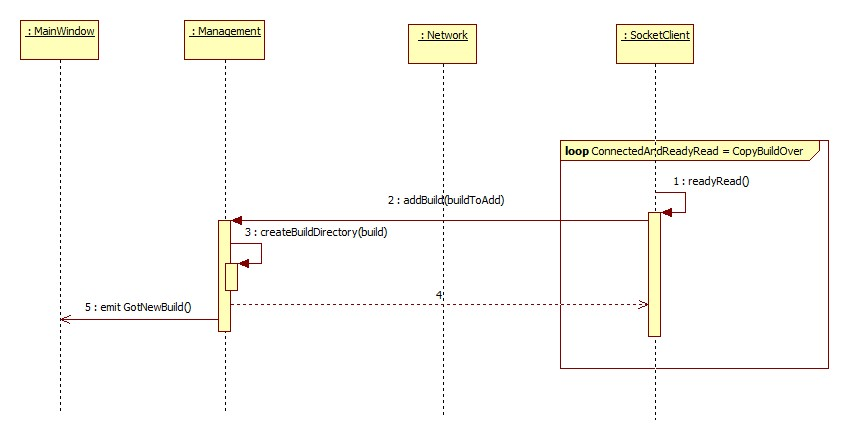
\includegraphics[scale=0.4]{CommunicationProtocol/SequenceDiagrams/Client/CopyOver.jpg} 
%\end{center}
%\begin{center}
%Sequence Diagram(For Master Application)
%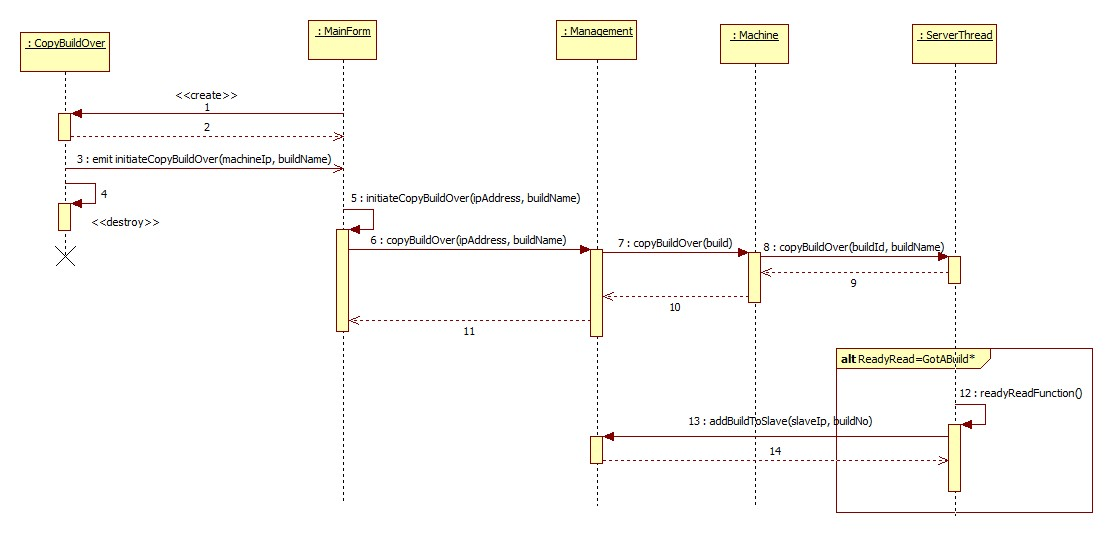
\includegraphics[scale=0.4]{CommunicationProtocol/SequenceDiagrams/Server/CopyOver.jpeg} 
%\end{center}
%%%%%%%%%%%%%%%%%%%%%%%
%%%%%%CopyOver			(End)
%%%%%%%%%%%%%%%%%%%%%%%



%%%%%%%%%%%%%%%%%%%%%%%
%%%%%%GetSysInfo		(Begin)
%%%%%%%%%%%%%%%%%%%%%%%
\subsection{GetSysInfo}
This protocol is used to obtain various system info from the slave machine to display on the master machine. The slave machine returns its "vitality" which is displayed on the master machine.
\begin{center}
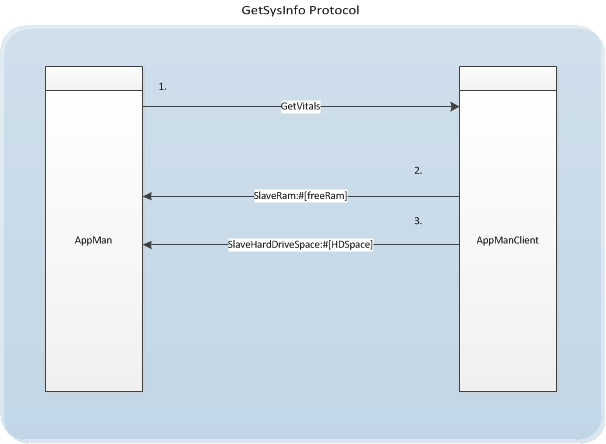
\includegraphics[scale=0.85]{CommunicationProtocol/GetSysInfoProtocol.jpg} 
\end{center}

%%%%%%%%%%%%%%%%%%%%%%%
%%%%%%GetSysInfo		(End)
%%%%%%%%%%%%%%%%%%%%%%%


%%%%%%%%%%%%%%%%%%%%%%%
%%%%%%SendBuild			(Begin)
%%%%%%%%%%%%%%%%%%%%%%%
\subsection{SendBuild}
This protocol is where a physical build is being sent to the slave machine. Before sending a build, the MD5 values are calculated for each and every file so that one can see what files are different. The MD5 values sent to the master will be used to create a CopyCompare class which will indicate which files will be sent across the network. The file that is sent across the network will be uncompressed and those files will be added in an uncompressed format on the AppManClient side.
\begin{center}
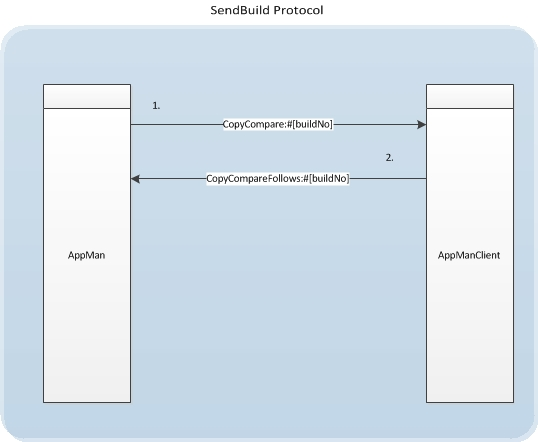
\includegraphics[scale=0.85]{CommunicationProtocol/SendBuildProtocol.jpg} 
\end{center}

%%%%%%%%%%%%%%%%%%%%%%%
%%%%%%SendBuild			(End)
%%%%%%%%%%%%%%%%%%%%%%%


\section{Functional Requirements}

\subsection{Use Case Diagrams}
\begin{itemize}
\item AppMan\\
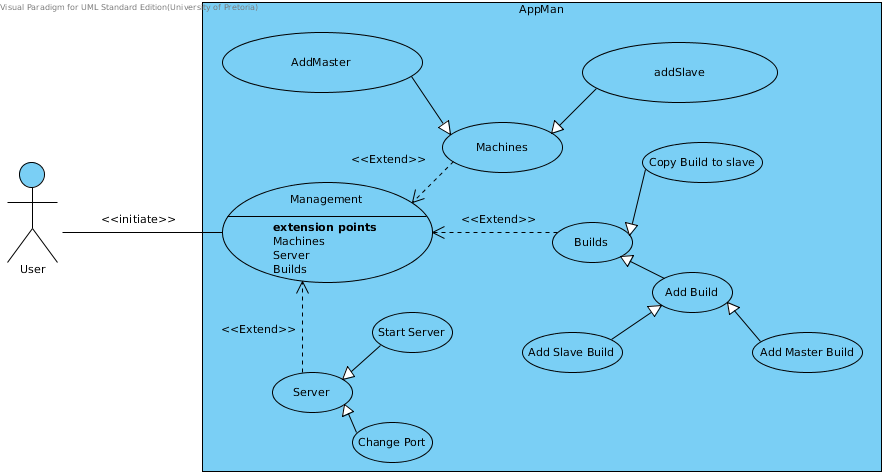
\includegraphics[angle = 90, scale=0.7]{UseCaseDiagram.png} 
\item AppManClient\\
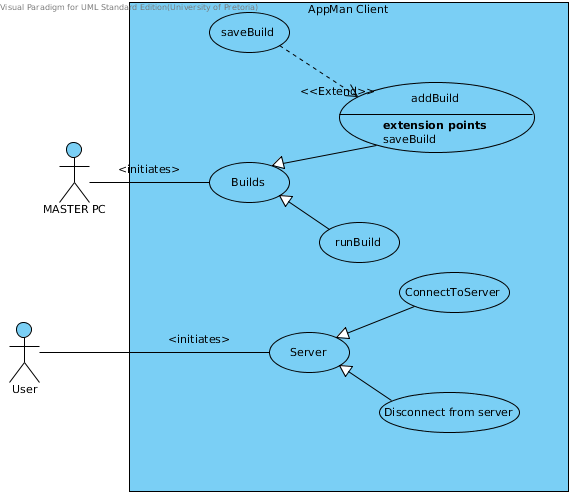
\includegraphics[angle = 90, scale=0.8]{UseCaseDiagramClient.png} 
\end{itemize}

\newpage
\subsection{Builds}
\begin{itemize}
\item Builds must be addable to the master
\item Builds must be updated on the slave computers once a change have been made
\item Only changed files must be sent to the slave computers once a change has been made
\item Easy to manage the builds that are on the master computer
\item Builds must be able to have the following
\begin{itemize}
\item Build Number
\item Directory
\item Name
\item Description
\end{itemize}
\end{itemize}

\subsection{Copying}
\begin{itemize}
\item Copying must be done over the network
\item The copy of multiple files must be compressed to reduce the time it takes to copy a file
\item Progress of copy must be shown on master computer while copying takes place
\end{itemize}

\subsection{User Interface}
\begin{itemize}
\item The user interface must be easy to use
\item The user interface must make use of drag and drop capabilities to promote usability
\end{itemize}

\subsection{Server \& Client Applications}
\begin{itemize}
\item The Applications must start on computer startup in a minimized form(e.g. in the tray)
\item The Master machine server must start on application start
\item Slave machines must connect to the master computer via the network once the application starts up
\item Slave machines must prompt connection details once and then connect automatically afterwards
\item The user interface must make use of drag and drop capabilities to promote usability
\end{itemize}

\section{Glossary}
\begin{itemize}
\item Build - An application build version that could potentially be distributed to slave computers
\item Slave - A computer that will be controlled via a master computer
\item Application builds will be sent to this computer
\item Master - A computer that will control Slaves across a network
\item Server - A machine waiting on the network for connections from other machines
\item GUI - Graphical User Interface with which a user can control an application
\item Project - This project. The distributed application manager
\item Application Configuration - Environment variables that are specified when running an application
\item Colour coding - The use of different colours to display certain information
\end{itemize}


\end{document}